\chapter{Grundlagen}\label{ch:grundlagen}

In diesem Kapitel werden die notwendigen Definitionen und Methoden erläutert,
die für das Verständnis der Arbeit von Bedeutung sind. Zunächst werden die
Ziele und Grenzen des Softwaretestens definiert. Dann folgt eine kurze
Einführung in den Begriff der Webanwendung und  die Erklärung des Konzeptes
der Testumgebung. Um mehr über die Vorteile der Automatisierung zu erfahren,
wird im nächsten Teil das Konzept der Testautomatisierung erläutert, gefolgt
von der Vorstellung verschiedener Testmethoden und -ansätze. Das Konzept des
Testens im Bereich der Softwareentwicklung ist umfangreich und kann in dieser
Arbeit nicht vollständig behandelt werden. Daher werden einige
Testarten am Ende vorgestellt.


\section{Ziele und Grenzen des Softwaretestens}

Die Standarddefinition des Testens nach dem
ANSI/IEEE 1059-Standard besagt, dass Testen der
Prozess der Analyse eines Softwareobjekts ist, um
Unterschiede zwischen bestehenden und erforderlichen
Bedingungen (d.h. Defekte/Fehler/Bugs) zu erkennen
und die Eigenschaften des Softwareobjekts zu bewerten (vgl. \cite{singh2012software}, S.07).
Das Softwaretesten ist daher eine Methode, um zu überprüfen,
ob das Softwareprodukt den erwarteten
Anforderungen entspricht und um sicherzustellen, dass
es frei von Fehlern ist.

Im 21. Jahrhundert ist der Einsatz von Software und
Anwendungen weit verbreitet und kein Bereich bleibt
davon verschont. Die Gesamtmenge der weltweit erstellten,
erfassten, kopierten und verbrauchten Daten ist laut
Statista (vgl. \cite{Statista2021}) bis 2020 rasant auf 64,2
Zettabyte \begin{math}(2^{70})\end{math} angestiegen. Die Nutzer vertrauen ihre sensiblen und privaten Daten
Plattformen an, deren Aufgabe ist es, sie zu schützen. Testen
ist wichtig, weil Softwarefehler teuer oder sogar gefährlich
sein können. Sie können finanzielle
und menschliche Verluste verursachen, und die Geschichte
ist voll von solchen Beispielen:

\noindent
\begin{enumerate}
    \item Im Mai 1996 führte ein Softwarefehler dazu, dass
     den Konten von 823 Kunden einer großen US-Bank 920
     Millionen US-Dollar gutgeschrieben wurden (vgl. \cite{Devi2015}).
    \item China Airlines Airbus A300 crashed due to a software bug on April 26,
     1994, killing 264 innocents live (vgl. \cite{Takeuch1996}).
\end{enumerate}

Das Testen einer Anwendung hat viele Vorteile. Zu den wichtigsten
gehören die folgenden:


 \textbf{Kosteneffektivität}: Das
rechtzeitige Testen eines IT-Projekts hilft auf
lange Sicht Geld zu sparen. Wenn die Fehler bereits in
der frühen Phase des Softwaretests entdeckt werden,
kostet es weniger, sie zu beheben. Es ist besser, mit
dem Testen früher zu beginnen und es in jeder Phase des
Lebenszyklus der Softwareentwicklung einzuführen.
Regelmäßige Tests sind erforderlich (vgl. \cite{kumar2010software}, S.53), um
sicherzustellen, dass die Anwendung gemäß den Anforderungen entwickelt wird.

\begin{figure}[H]
    \centering
    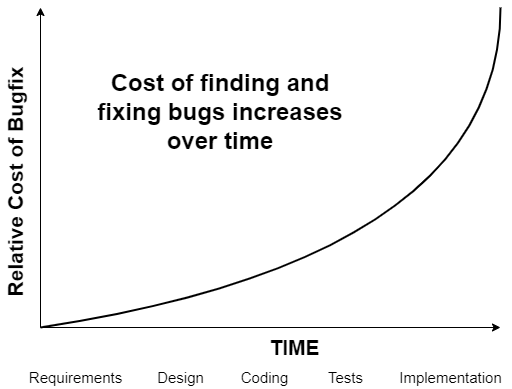
\includegraphics[scale=0.5]{images/Cost-of-fixing-bugs-in-different-phases}
    \caption{Kosten für die Behebung von Fehlern (Bugs) in verschiedenen Phasen (vgl. \cite{kumar2010software})} \label{fig:mof}
\end{figure}


\textbf{Erhöhung der Sicherheit}: Sicherheit ist der anfälligste und
sensibelste Teil des Softwaretestens. Durch Testen wird sichergestellt,
dass die Anwendung über einen minimalen Schutz verfügt. Testen hilft
dabei, Risiken und Probleme früher zu beseitigen. So wird die Anwendung für Nutzer attraktiv,
die vertrauenswürdige Produkte suchen (vgl. \cite{shultz2011software}, S.09).

\textbf{Produktqualität}: Sie ist eine wesentliche
Voraussetzung für jedes Softwareprodukt. Zu den sechs Gruppen von Software-Qualitätsindikatoren
in der ISO-Norm 9126 (vgl. \cite{AlainAbran2010}) gehört die Wartbarkeit, zu der auch die Untergruppe Testbarkeit gehört.
Durch Testen kann die Qualität einer Anwendung sowie ihre Wartbarkeit erhöht werden und so wird dem Kunden sichergestellt,
dass ein Qualitätsprodukt geliefert wird.


Aus diesen Gründen ist das Testen von Software ein
integraler Bestandteil des Softwareentwicklungsprozesses, jedoch hat es Grenzen.
Testen dient nur dazu, das Vorhandensein von potentiellen Fehlern
aufzudecken. Aber es kann nicht sicherstellen, dass
die Software keine Fehler oder Bugs enthält (vgl. \cite{kumar2010software}, S.55).
Dazu können Tests nicht nachweisen, dass ein Produkt unter allen
Bedingungen richtig funktioniert, sondern nur, dass es unter
bestimmten Bedingungen nicht richtig funktioniert (vgl. \cite{kumar2010software}, S.56).



Da das Ziel dieser Arbeit darin besteht, eine \Gls{TestSuite} für
eine Webanwendung einzurichten, ist es wichtig zu
definieren, was mit Webanwendung eigentlich gemeint ist.

\section{Webanwendungen}

Das weite Feld der Softwareentwicklung umfasst auch die
Entwicklung von Webanwendungen. Lange Zeit wurden
Anwendungen als kompakte, installierbare Programme
verkauft. Dabei handelt es sich um die so genannten
klassischen Anwendungen oder Computeranwendungen, die
lokal auf einem Computer, Mobiltelefon oder Tablet
installiert werden müssen. Im Gegensatz zu herkömmlichen
Anwendungen werden Webanwendungen nicht lokal auf dem Gerät
des Nutzers installiert, sondern auf einem Server, so dass
sie über eine bestimmte \acs{url} zugänglich sind.

Nach Kappel et al. ist eine Webanwendung ein Softwaresystem,
das auf den Spezifikationen des World Wide Web Consortiums
(\acs{w3c}) basiert und Webressourcen bereitstellt, die über
eine Benutzeroberfläche wie einen Webbrowser genutzt werden
können (vgl. \cite{kappel1}, S.02).

Für den Betrieb einer Webanwendung werden mehrere
Computersystemkomponenten benötigt.Erstens das \gls{frontend},
das die grafische Oberfläche bezeichnet, mit der der
Benutzer interagiert, gefolgt vom \gls{backend}, das die
Logik der Anwendung enthält (z.B Datenbanken, Cloud).


Der Benutzer greift auf die Webanwendung über einen Computer
zu, der als Client bezeichnet wird. Der Client sendet eine
oder mehrere Anfragen über das Internet oder Intranet via
\acs{http} oder \acs{https}  an einen anderen Computer (Server),
auf dem die Webanwendung läuft. Der Server nimmt dann die
HTTP-Anfragen entgegen und verarbeitet sie. Je nach Anfrage
werden die angeforderten Daten entweder aus der Datenbank
abgerufen oder gespeichert. Die verarbeiteten Daten werden
dann vom Server in einer entsprechenden Antwort
(HTTP-Response) an den Client zurückgesendet und im
Webbrowser angezeigt. So funktionieren Webanwendungen grundsätzlich.

Um Webanwendungen zu testen, ist es wichtig, eine Testumgebung zu schaffen.
Diese Testumgebung ermöglicht es dem Tester, alle möglichen Schwachstellen in einer Webanwendung zu untersuchen,
ohne die Anwendung zu gefährden, wenn sie bereits in Produktion ist.


\section{Testumgebung}
\section{Testautomatisierung}

Nach Sharma et al. ist die Testautomatisierung eine Technik,
bei der Skripte geschrieben werden, um einen manuellen
Testprozess zu automatisieren (vgl. \cite{sharma2014web}, S.909). Bei der
Testautomatisierung werden vordefinierte Tests durchgeführt,
um verschiedene Funktionen in einer Anwendung zu überprüfen.
Dies bedeutet, dass Tools und Testskripte verwendet werden, um verschiedene
Zustände zu erzeugen und Daten vorzubereiten. Anschließend wird eine
Reihe von Schritten ausgeführt, um ein Szenario zu validieren.
Auf diese Weise können die Tester feststellen, ob eine Anwendung
wie erwartet funktioniert oder nicht. Entwicklungs- und Testteams
entscheiden sich aus mehreren Gründen für die Testautomatisierung.
Zu den wichtigsten gehören:

\textbf{Zeit}: Manuelle Tests sind langsam und können mit vielen Entwicklungsprozessen
nicht mithalten (vgl. \cite{sharma2014web}, S.910).


\textbf{Kosten}: Manuelle Tests sind ressourcenintensiv und kostspielig
(vgl. \cite{sharma2014web}, S.910).


\textbf{Genauigkeit}: Manuelle Tests sind bei der Durchführung sich wiederholender
Aufgaben fehleranfällig. Umgekehrt verringert die Automatisierung die
Wahrscheinlichkeit dieser Fehler (vgl. \cite{sharma2014web}, S.910).


\textbf{Umfang}: Bei der Durchführung komplexer Iterationen ist es schwierig,
sich auf manuelle Tests zu verlassen (vgl. \cite{sharma2014web}, S.910).


Laut dem Global Quality Report profitieren Unternehmen auf unterschiedliche
Weise von automatisierten Tests. Rund 60\% der Unternehmen gaben an,
dass sich die Fähigkeit zur Erkennung von Anwendungsfehlern durch eine höhere
Testabdeckung verbessert hat (vgl. \cite{Buenen201718}, S.30). Weitere 57\% stellten fest, dass die Wiederverwendung von Testfällen nach
dem Einsatz der Automatisierung zunahm. Gleichzeitig verzeichneten 54\%
eine Verringerung des Zeitaufwands für
Testzyklen (vgl. \cite{Buenen201718}, S.31).

\begin{figure}
    \centering
    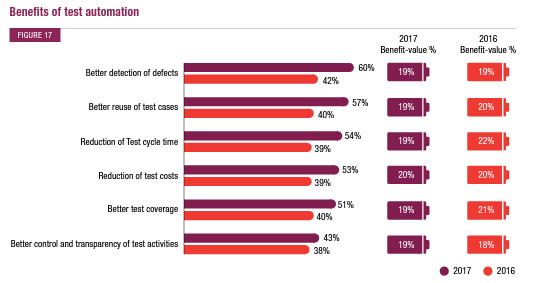
\includegraphics[scale=1.3]{images/benefits_of_test_automation}
    \caption{Vorteile der Testautomatisierung (vgl. \cite{Buenen201718}, S.31)} \label{fig:mof}
\end{figure}

In den folgenden Abschnitten werden die verschiedenen Arten von Tests
behandelt. Diese Tests können sowohl manuell als auch automatisch
durchgeführt werden. Da der Schwerpunkt dieser Arbeit auf der
Automatisierung liegt, wird nur dieser Aspekt betrachtet.

\section{Testsmethoden und -ansätze}

Softwareobjekte können auf unterschiedliche Weise
getestet werden. Generell wird zwischen statischen und
dynamischen Tests unterschieden. In den folgenden
Fällen werden beide Konzepte in den folgenden
Abschnitten ausführlicher dargestellt.

\subsection{Statisches Testen}

Statisches Testen ist eine Softwaretestmethode,
bei der ein Programm zusammen mit den zugehörigen
Dokumenten untersucht wird, ohne dass das Programm
ausgeführt werden muss. Konkret besteht der Prozess aus
der Prüfung schriftlicher Dokumente, die insgesamt
einen Überblick über die zu testende Softwareanwendung
geben. Zu den geprüften Dokumenten gehören
Anforderungsspezifikationen, Designdokumente,
Benutzerdokumente, Webseiteninhalte, Quellcode,
Testfälle, Testdaten und Testskripte,
Benutzerdokumente, Spezifikations- und
Matrixdokumente. Statische Tests erleichtern die
Kommunikation zwischen den Teams und vermitteln
einen besseren Eindruck von den Qualitätsproblemen
in der Software. Es reduziert nicht nur die Kosten
in den frühen Entwicklungsphasen (in Bezug auf die
Menge an Arbeit, die neu gemacht werden muss, um
eventuelle Fehler zu korrigieren), sondern auch die
Entwicklungszeit.

\subsection{Dynamisches Testen}

Dynamisches Testen ist eine Methode zur Bewertung
der Durchführbarkeit eines Softwareprogramms durch
Eingabe und Prüfung der Ausgabe. Die dynamische Methode
erfordert, dass der Code kompiliert und ausgeführt
wird. Dynamische Tests werden in zwei Kategorien unterteilt:
Whitebox- und  Blackboxtestverfahren.

\textbf{Whitebox-Testverfahren}

Whitebox-Testen ist eine Softwaretestmethode, bei
der dem Tester die interne Struktur/das Design
bekannt ist. Das Hauptziel  vom Whitebox-Testen ist
die Überprüfung der Korrektheit der Software
Anweisungen, Codepfade, Bedingungen, Schleifen
und Datenflüsse. Dieses Ziel wird oft als logische
Abdeckung bezeichnet (vgl. \cite{shultz2011software}, S.107).


\textbf{Blackbox-Testverfahren}

Blackbox-Testen ist eine Testmethode, bei der die
interne Struktur/der Code/das Design dem Tester nicht
bekannt ist. Das Hauptziel dieses Tests ist es, die
Funktionalität des zu testenden Systems zu überprüfen,
und diese Art von Tests erfordert die Ausführung der
kompletten Testsuite (vgl. \cite{shultz2011software}, S.112).


Die Blackbox-Methode ist diejenige, die in dieser
Arbeit entwickelt wird. Sie selbst ist in mehrere
Arten unterteilt, auf die im nächsten Kapitel
eingegangen wird.




\section{Verschiedene Testarten}
\section{Verschiedene Schritte zur Erstellung einer Testsuite}\label{sec:verschiedene-schritte-zur-erstellung-einer-testsuite}

In der heutigen wettbewerbsorientierten und schnelllebigen
Welt ist das Internet zu einem integralen Bestandteil des Lebens
geworden. Heutzutage treffen die meisten ihre Entscheidungen,
indem sie im Internet nach Informationen suchen. Das Hosten einer
Website ist daher nicht mehr optional, sondern f\"ur alle Arten von
Unternehmen obligatorisch. Es ist der erste Schritt, um auf dem
Markt relevant zu werden und zu bleiben. Es reicht nicht mehr aus,
nur eine Website zu haben. Ein Unternehmen muss eine Website
entwickeln, die informativ, zug\"anglich und benutzerfreundlich ist.
Um all diese Qualit\"aten zu erhalten, sollte die Website getestet
werden, und dieser Prozess des Testens einer Website ist als Web-Testing
bekannt. Um diese Aufgabe zu bew\"altigen,
durchlaufen die Testerteams mehrere Schritte:

\textbf{Erstellung eines Testplan:} Ein Testplan ist ein Dokument, das den
Umfang, die Vorgehensweise und den Zeitplan der geplanten Testaktivit\"aten
festlegt (vgl. \cite{shultz2011software}, S. 79). Das Hauptziel eines Testplans
ist die Erstellung einer Dokumentation, die beschreibt, wie der Tester
\"uberpr\"uft, ob das System wie vorgesehen funktioniert. Das Dokument sollte
beschreiben, was getestet werden muss, wie es getestet werden soll und wer
daf\"ur verantwortlich ist. Er ist die Grundlage f\"ur jede Testarbeit
(vgl. \cite{shultz2011software}, S. 79). Der Testplan enth\"alt in der Regel die
folgenden Informationen:

\begin{enumerate}
    \item Das Gesamtziel des Testaufwands.
    \item Einen detaillierten \"uberblick \"uber die Art und Weise, wie die Tests
    durchgef\"uhrt werden.
    \item Die zu pr\"ufenden Funktionen, Anwendungen oder Komponenten.
    \item Detaillierte Zeit- und Ressourcenzuweisungspl\"ane f\"ur Tester und
    Entwickler w\"ahrend aller Testphasen.
\end{enumerate}

\textbf{Erstellung einer Teststrategie :} Die Teststrategie beim Softwaretesten
ist definiert als eine Reihe von Leitprinzipien, die das Testdesign
bestimmen und regeln, wie der Softwaretestprozess durchgef\"uhrt wird. Das Ziel
der Teststrategie ist es, einen systematischen Ansatz f\"ur den
Softwaretestprozess zu liefern, um die Qualit\"at, R\"uckverfolgbarkeit,
Zuverl\"assigkeit und bessere Planung zu gew\"ahrleisten. Die
Teststrategie wird sehr oft mit dem Testplan verwechselt. Es gibt jedoch einen
bemerkenswerten Unterschied zwischen den beiden. Der Testplan konzentriert
sich auf die Organisation und das Management der Ressourcen sowie die
Definition der Ziele, w\"ahrend die Teststrategie sich auf die Umsetzung und die
Testtechniken konzentriert. Beide helfen bei der Planung, aber auf
unterschiedlicher Ebene.

\textbf{Testentwurf und implementierung :} Der Testentwurf ist ein Prozess,
der beschreibt, ``wie'' die Tests durchgef\"uhrt werden sollen und das
Schreiben von Testsuiten f\"ur das Testen einer Software. Er umfasst Prozesse
zur Identifizierung von Testf\"allen durch Aufz\"ahlung von Schritten der
definierten Testbedingungen. Die in der Teststrategie oder dem Testplan
definierten Testtechniken werden f\"ur die Aufz\"ahlung
der Schritte verwendet (vgl. \cite{shultz2011software}, S. 46).



Je nach den Zielen, die im Testplan festgelegt wurden, konzentrieren sich die
Entwickler auf bestimmte Arten von Tests, z. B. Funktionale Tests,
Performancetests oder Sicherheitstests. F\"ur diese Arbeit wurde vorab ein
Testplan erstellt. Aus diesem Grund wird der Schwerpunkt auf der Implementierung
von Tests und der Einrichtung der Testinfrastruktur liegen.



